\subsubsection{Real photons}
%Contributed by Klaus Reygers, Ana Marin, Dmitri Peresunko

Recently, ALICE has measured direct photon spectra in three centrality classes in \PbPb collisions at $\sqrtsNN=\unit[2.76]{\UTeV}$ \cite{Adam:2015lda}. 
An excess of direct photons
%above the decay photon spectrum 
was quantified by the $\pT$ dependent double ratio
\begin{equation}
  \label{eq:doubleratio}
  R_{\PGg}  \equiv \left . \frac{\PGg_{\mathrm{incl}}}{\PGpz_{\mathrm{param}}} \right / \frac{\PGg_{\mathrm{decay}}}{\PGpz_{\mathrm{param}}}
 = \frac{\PGg_{\mathrm{incl}}}{\PGg_{\mathrm{decay}}}, 
\end{equation}
where $\PGg_{\mathrm{incl}}$ is the measured inclusive photon spectrum, $\PGpz_{\mathrm{param}}$ a parametrization of the measured $\PGpz$ spectrum, and $\PGg_{\mathrm{decay}}$ the calculated decay photon spectrum. The double ratio has the advantage that some of the largest systematic uncertainties cancel partially or completely. 
%Using the double ratio, the direct photon yield  can be calculated from the inclusive photon yield as
%\begin{equation}\label{eq:subs}
%  \gamma_{\mathrm{direct}} = \gamma_{\mathrm{incl}}-\gamma_{\mathrm{decay}} = (1- \frac{1}{R_\gamma})\cdot \gamma_{\mathrm{incl}}.
%\end{equation}
The measurement combines results of the Photon Conversion Method (PCM) and of the Photon Spectrometer (PHOS), see Fig.~\ref{fig:RealPhotonsRg}, left. In central collisions at low $\pT  < \unit[3-4]{\UGeVc}$ an excess with respect to prompt photon predictions is observed that is attributed to thermal photon emission from the QGP. For the most central 0--20\% centrality the low \pT{} excess is of the order of 10--15\%, while the total uncertainty of the order of 6\%. A signal of direct photons was found in central collisions, but on the level of $\sim 2\sigma$, while in mid-central and especially in peripheral the significance is even smaller. On the other hand, peripheral collisions are important since there one can estimate and restrict the contribution from prompt direct photons.  

%-----------------------------------------------------------------------%
\begin{figure}[hbt]
\centering
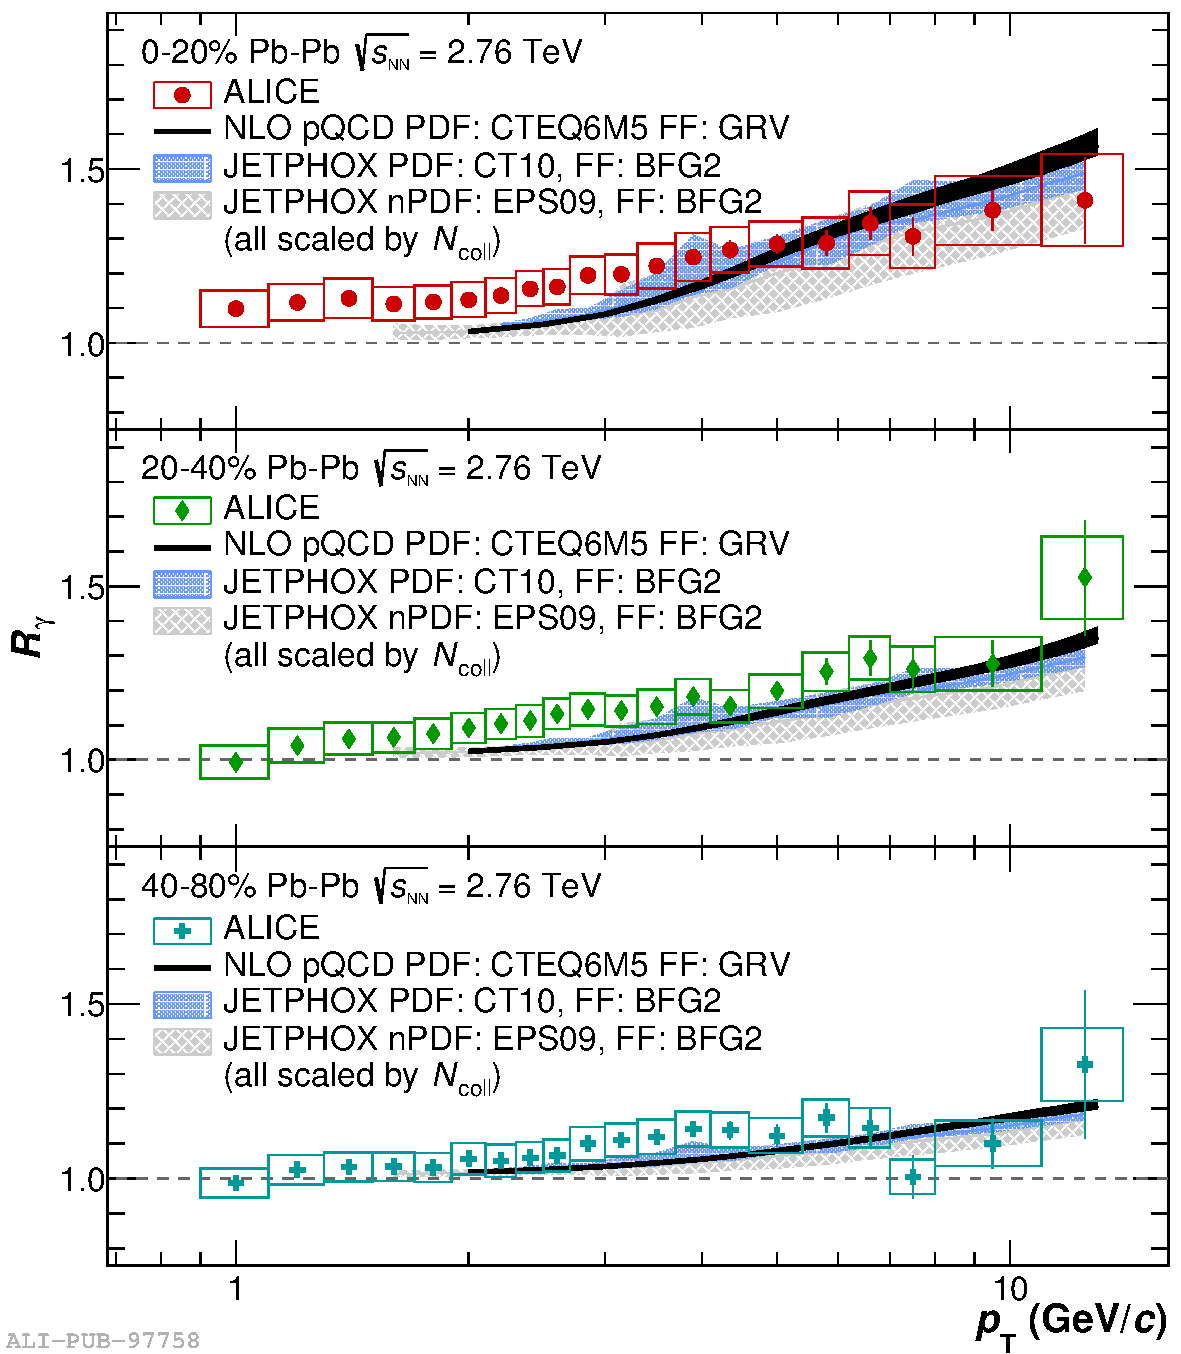
\includegraphics[width=0.46\textwidth]{\main/thermalradiation/figs/2015-Sep-24-DR_combMeasurement_incNLO.pdf}
\hfill
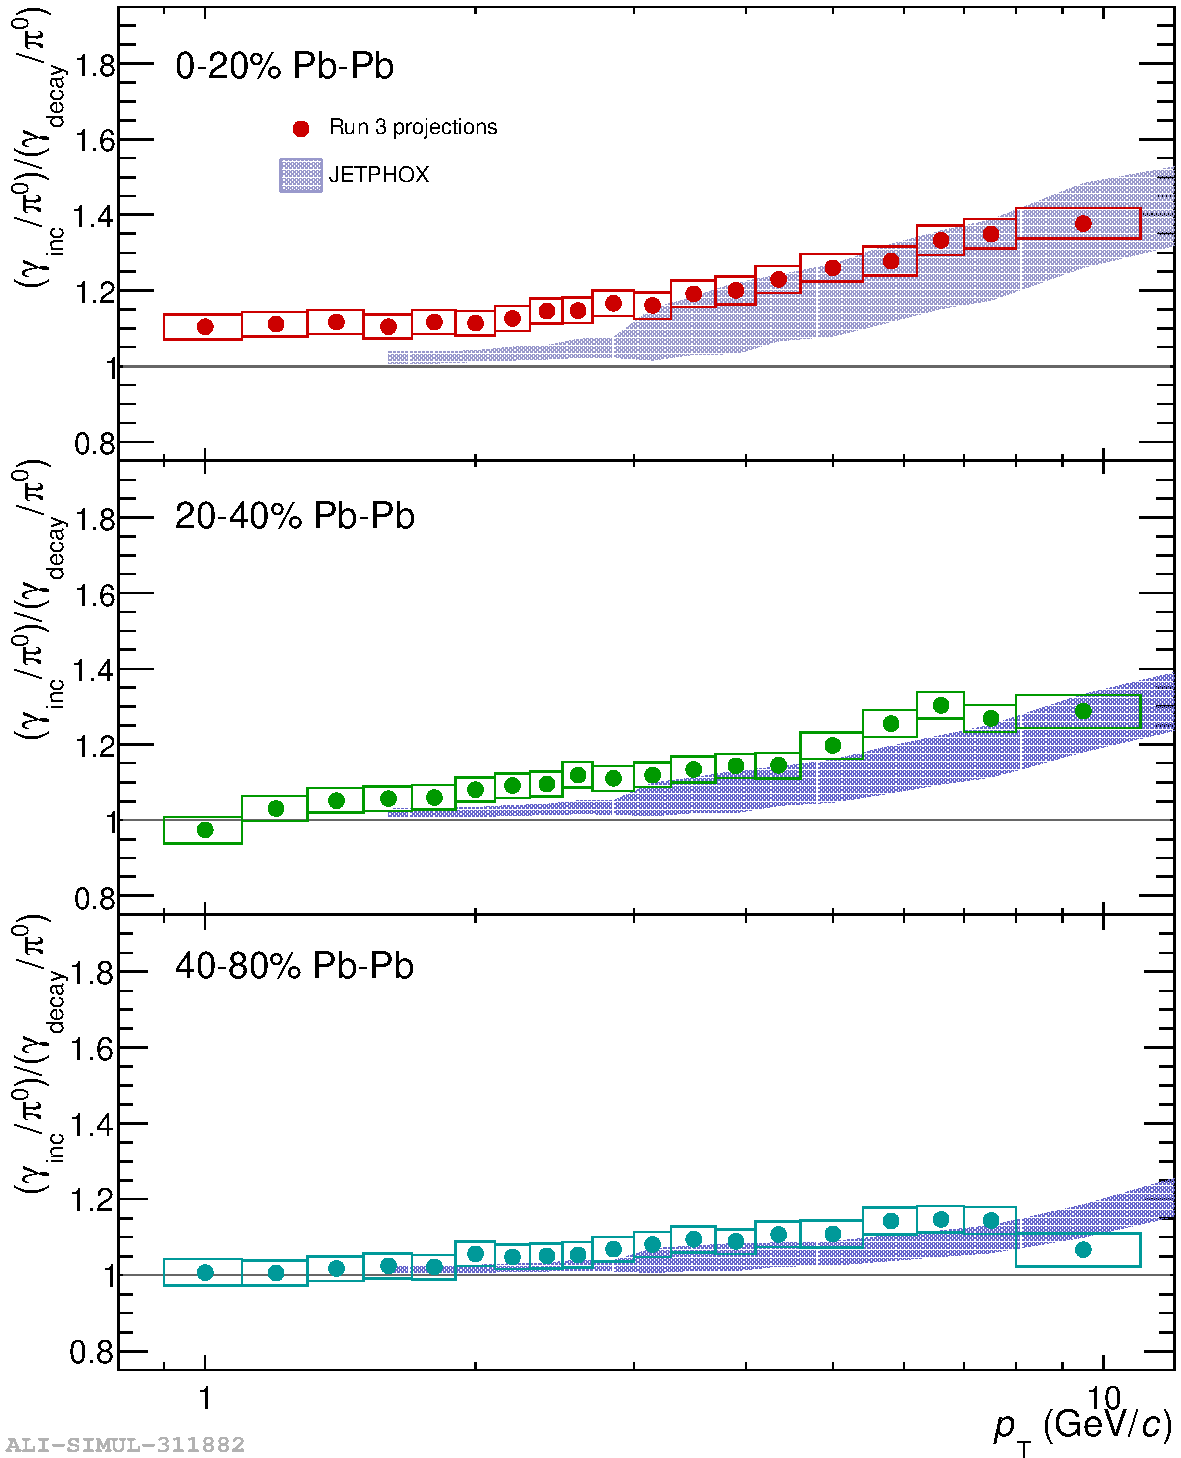
\includegraphics[width=0.425\textwidth]{\main/thermalradiation/figs/2018-10-10-2018-10-10-ReducedRg.pdf}
\caption{$R_{\PGg}$ measured \cite{Adam:2015lda} (left) and $R_{\PGg}$ projected keeping the measured values of $R_{\PGg}$ and recalculating the uncertainties as explained in the text.}
\label{fig:RealPhotonsRg}
\end{figure}
%-----------------------------------------------------------------------%

For Run 3 the PCM measurement will be influenced by the ALICE Inner Tracking System (ITS) and Time Projection Chamber (TPC) upgrades, while PHOS and the Electromagnetic Calorimeter (EMCal) will be kept unchanged. 
The new ITS shows an improved low \pT{} tracking efficiency and its material thickness is reduced by approximately 30\%. Two \unit[1]{\Umm} tungsten wires with well known thickness will be installed parallel to the beam direction. 
%The wires will be positioned between layers 2-3 and 4-5 at R = 4-14 cm and R = 30.9 cm, being inclined the most inner one. 
The TPC continuous readout mode together with large pile-up may prevent on the other hand the use of photon conversions beyond a radius of \unit[35]{\Ucm}. These will translate
into a ~35\% lower photon efficiency. On the other hand, the PCM measurement will also profit from the dedicated heavy-ion run with reduced magnetic field of the ALICE solenoid, that increases considerable the low \pT{} reconstruction efficiency.
To estimate how one can improve accuracy of our measurement, we split uncertainties into 3 classes: those which can be improved with increase of statistics (statistical uncertainties, uncertainties related to \PGpz spectrum extraction, $\PGh/\PGpz$ ratio); uncertainties which can be reduced using new techniques and some special methods (material budget estimate - with calibrated material analysis, energy scale in calorimeters with new hybrid \PGpz methods); and uncertainties related to the properties of the detector which can not be improved (hadron contamination in calorimeters, electron identification in conversion method etc.). To estimate the improvement of the uncertainties we assumed that the available statistics will increase by a factor of 100. 
%The main contributor to the systematic uncertainties at 
%low \pT\  for PCM is the material budget uncertainty with 4.5\%. 
The major improvement foreseen for Run 3 is the used of the calibrated tungsten wires
inserted in the ITS to determine the product of the photon flux times the \PGg reconstruction efficiency. This product would then be used to precisely determine the material thickness in the rest of the ITS (assuming $\varphi$-independent photon flux and taking the radial dependence of the reconstruction efficiency from simulation).
The proposed calibration method is based on weights calculated 
as the double ratio: 
\begin{equation}
\omega_i= 
{\left(\frac{N_{\PGg}^{\rm rec}(r_i)}{N_{\PGg}^{\rm rec}(r_{\rm wire})}\right)^{\rm data}} /
{\left(\frac{N_{\PGg}^{\rm rec}(r_i)}{N_{\PGg}^{\rm rec}(r_{\rm wire})}\right)^{\rm MC}} 
\end{equation}
where $N_{\PGg}^{\rm rec}(r_i)$ and $N_{\PGg}^{\rm rec}(r_{\rm wire})$ are the number of reconstructed \PGg 's in data or in MC simulations in a given radial bin and the calibrated wire, respectively.
%These weights are then used to scale the reconstruction efficiency in each radial bin of the detector.
This procedure is being implemented for Run 2 data using the TPC gas as calibration material. First results show that a systematic uncertainty of 1.8\% can be achieved. For the Run 3 projections a systematic uncertainty of 1\% on the ITS thickness is taken. The uncorrelated systematic uncertainties on the \PGpz and \PGh measurements will be reduced by a factor 10 due to the increased luminosity. The systematic uncertainties on photon selection and particle identification are expected to be reduced by 50\%.
Figure~\ref{fig:RealPhotonsRg} (right) shows the projection on the $R_{\PGg}$ measurement 
for Run 3 calculated with these assumptions: we keep measured values of $R_{\PGg}$ but re-calculate uncertainties. The total errors are reduced by $\sim50$\%. In addition to reductions of uncertainties, the large statistics foreseen for Run 3 will allow to explore the 0--1\% centrality. 

%{\bf Compare of different predictions Rg, with expected uncertainties: can we distinguish theories? Can we establish direct (thermal) photon measurements with 5 sigma? (Ana collect predictions and make Rg for 5 TeV, Cocktail: 5 TeV prelim pi0+eta/pi0 from 2.76)

%To which extend should we reduce sys/stat uncertainties to reach 5 sigma? Use our code.
%}

%Observation of the collective flow of final hadrons was one of the most important findings in the area of heavy-ion collisions.
%Collective flow is the azimuthal asymmetry in particle production, common for all soft particles in the collision. 
%It is interpreted as a collective expansion of initially spatially asymmetric hot matter. This initial deformation is the result of partial overlap of colliding nuclei in non-central collisions.  Transforming the initial geometric asymmetry into the asymmetry of momentum distribution of final particles requires strong interaction between particles of the matter, therefore hydrodynamic-like models provide very good description of this effect. 
%Direct photons do not interact with hot matter and deliver information about the collective  flow at the moment of their emission. As hydrodynamic models predict, photons emitted at the initial stage by hot quark-gluon matter carry very small collective flow since it is not developed yet at this stage. In contrast, direct photons emitted at the latest stage of hadron gas expansion carry much larger collective flow, similar to one of final hadrons. 
%Averaging over the whole history of the collision leads to the prediction of direct photon flow considerably smaller than one of final hadrons. 
%However, the first measurements of direct photon elliptic flow $v_{2}$ performed by PHENIX experiment \cite{Adare:2011zr}, demonstrated that the direct photon flow is comparable with one of final hadrons and much larger than one predicted by hydrodynamic models. 

%-----------------------------------------------------------------------%
\begin{figure}[htb]
\centering
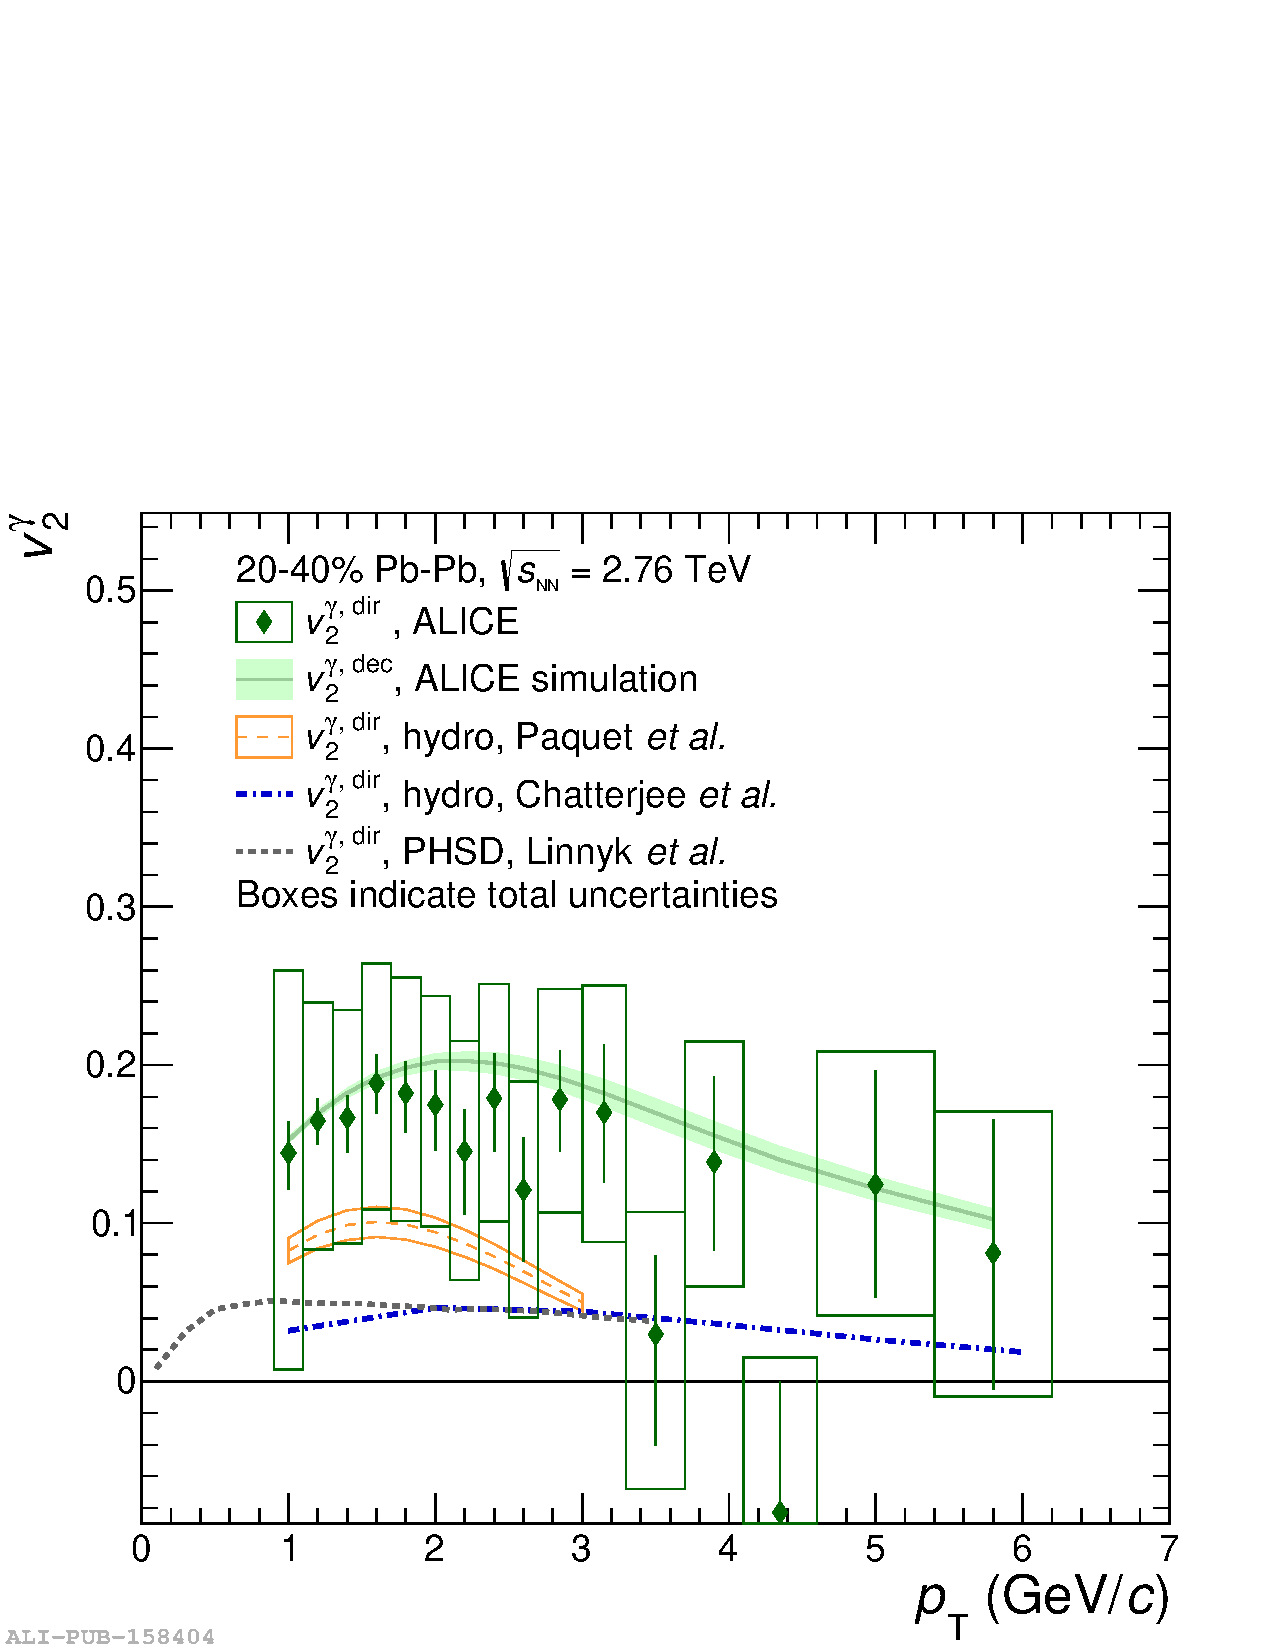
\includegraphics[width=0.45\textwidth]{\main/thermalradiation/figs/2018-May-11-2040_v2dir_combined_theory}
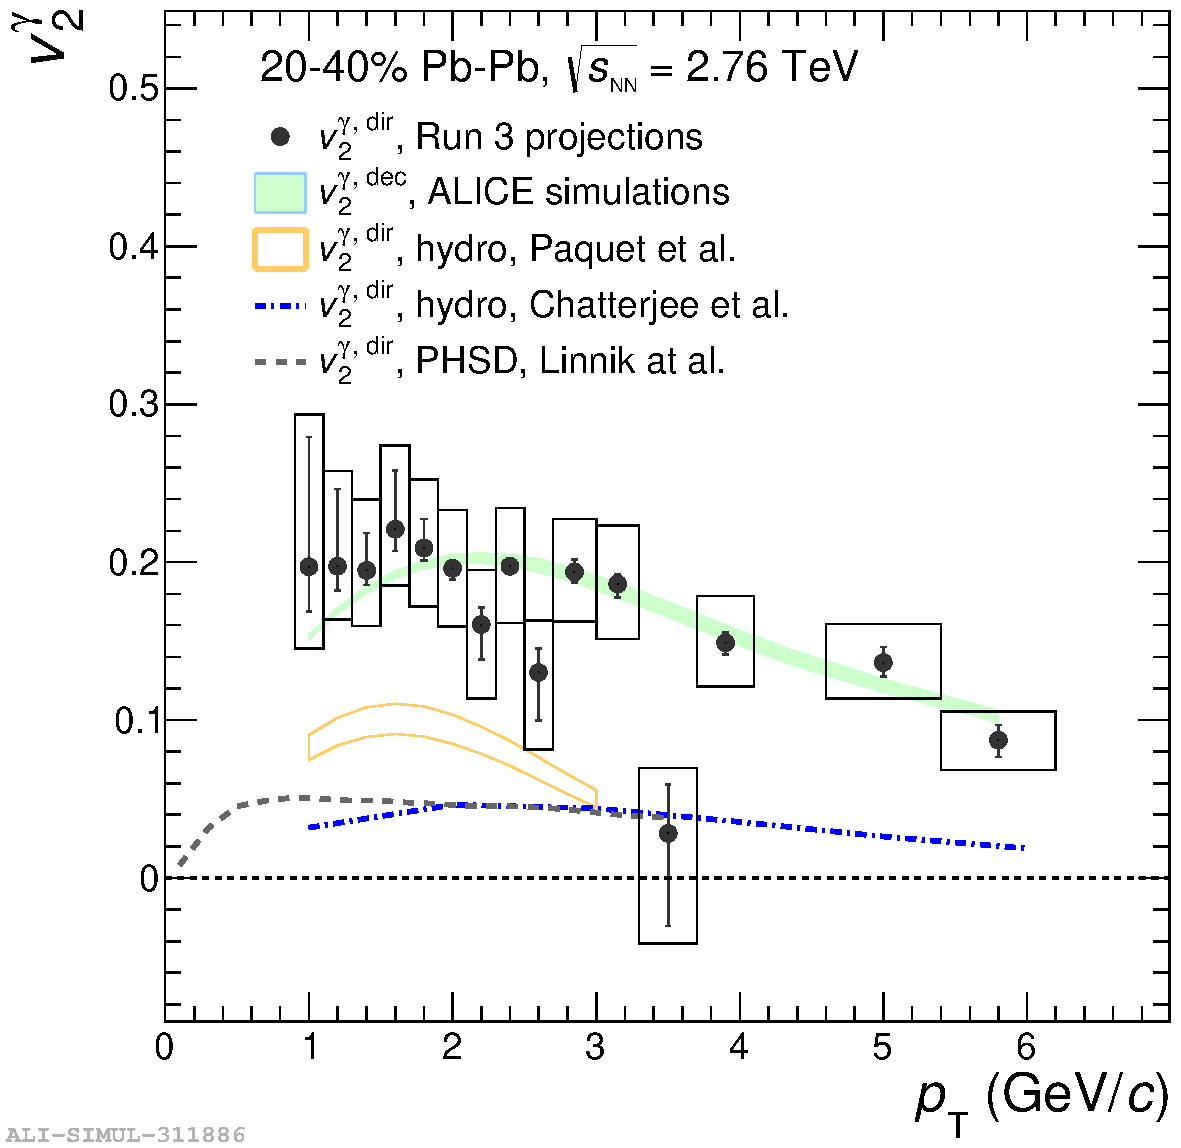
\includegraphics[width=0.42\textwidth]{\main/thermalradiation/figs/2018-10-10-2018-10-10-ProjectionV2.pdf}
\caption{Direct photon flow in mid-central collisions. Left: direct photon collective flow measured in \PbPb{} collisions compared to decay photon flow and several theoretical predictions. Right: expected accuracy in Run 3 keeping the  measured values of $R_{\PGg}$ and $v_{2}^{\PGg}$ and recalculating the uncertainties as explained in the text. }
\label{fig:RealPhotonsV2dir}
\end{figure}
%-----------------------------------------------------------------------%

ALICE performed measurements of the direct photon elliptic flow \cite{Acharya:2018bdy} in \PbPb{} collisions at $\sqrtsNN=\unit[2.76]{\UTeV}$ for the two centrality classes, 0--20\% and 20--40\%, see Fig.~\ref{fig:RealPhotonsV2dir}, left plot for 20--40\% centrality.
The measured direct photon elliptic flow $v_2^{\PGg,\rm dir}$ is compared to the estimated decay photon elliptic flow $v_2^{\PGg,\rm dec}$, marked as cocktail, and to the predictions of several theoretical models. Similar to RHIC measurements, the direct and decay photon elliptic flow are very close and systematically higher than theoretical predictions of hydrodynamic  \cite{Gale:2014dfa,Chatterjee:2017akg} and the transport  \cite{Linnyk:2015tha} models. However, because of the large uncertainties  one can not presently exclude neither of theoretical calculations. Using the same assumption concerning photon and neutral measurements in Run 3 as for $R_{\PGg}$, we estimated expected accuracy of $v_2^{\PGg,\rm dir}$ measurements in Run 3. We keep mean values the same but reduce uncertainties as expected, see Figure~\ref{fig:RealPhotonsV2dir} (right). shows the projection on the $v_2^{\PGg}$ measurement 
for Run 3. Similar to $R_{\PGg}$ with the current assumptions the total errors will be reduced by factor $\sim$ 2 and one will be able to exclude or confirm available theoretical calculations.
%{\bf We estimated v2dir with updated Rg uncertainties}





%\begin{itemize}
%\item First measurement at LHC from soft exponential component of photon pT spectrum (ALICE, Phys.Lett. B754 (2016) 235): T ~ 300 MeV (effective temperature averaged over system evolution)
%\item "Photon puzzle"
%\item Projections for Run3/4 in preparation: reduce systematic error (material budget uncertainty)
%\end{itemize}
